\documentclass[hyperref={pdfpagelabels=false}]{beamer}
\mode<presentation>

% Packages
\usepackage[utf8]{inputenc}
\usepackage[T1]{fontenc}
\usepackage[portuges]{babel}
\usepackage{amsmath, amssymb, mathtools, mathrsfs}
\usepackage{graphicx}
%\usepackage{subfig}
\newcommand{\nologo}{\setbeamertemplate{logo}{}}
\usepackage{textcomp}
\usepackage{comment}
\usepackage{float}
\usepackage{nicefrac}
\usepackage[labelformat=empty]{caption}
%\usepackage{subfig}
\usepackage{notoccite}
\usepackage{lmodern}
\usepackage{tikz}
\usetikzlibrary{arrows} %Pacotes necessários para o Tikz
\usetikzlibrary{patterns} %Pacotes necessários para o Tikz
%\usepackage{subfigure}
\usepackage{subcaption}

% Definição e operadores auxiliares
\DeclareMathOperator*{\argmin}{arg\,min}
\DeclareMathOperator*{\argmax}{arg\,max}

% Preâmbulo
\title[PDS]{Processamento Digital de Sinais - Sistemas no Tempo Discreto}
\author[Edmar Candeia Gurj\~{a}o]{Edmar Candeia Gurj\~{a}o}
\institute[UFCG/CEEI/DEE]{Universidade Federal de Campina Grande}
\date{09 de maio de 2017}

% Definição dos ambientes para Definção, Teorema e Lema.
\newtheorem{Defini\c{c}\~{a}o}{Definicao}
\newtheorem{Teorema}{Teorema}
\newtheorem{Lema}{Lema}

% Configurações Visuais do Texto
\usetheme{CambridgeUS}
\usecolortheme{seahorse}
\usecolortheme{rose}
\usefonttheme[onlysmall]{structurebold}
\setbeamercolor{title}{fg=blue!15!black}
\usefonttheme[onlylarge]{structuresmallcapsserif}
\usefonttheme[onlysmall]{structurebold}
\setbeamercolor{alerted text}{fg=blue!80!black}
\beamertemplatetransparentcovereddynamicmedium

\begin{document}	
	
\logo{
\includegraphics[height=0.8cm]{Figuras/UFCG_logo}}

\begin{frame}[c, allowframebreaks]
	\titlepage
\end{frame}

\section{Representações para Sistemas no Tempo Discreto}

%\subsection{Introdu\c{c}\~{a}o}


\begin{frame}[c, allowframebreaks]

\begin{itemize}
\item Vamos estudar formas de representar um sistema no tempo discreto, com entrada $x[n]$ e saída $y[n]$, relacionadas por uma equação de diferença, por exemplo
\[
y[n] - ay[n-1] = b_0x[n] + b_1x[n-1]
\]
\item E para tanto vamos utilizar as estruturas básicas 
\begin{figure}[H]
	\includegraphics[scale = 0.4]{Figuras/Figura61Oppenheim2aEdicao}
\end{figure}
\end{itemize}
\end{frame}
\end{document}

%%%
\begin{frame}[c, allowframebreaks]

\begin{itemize}
\item Então
\[
X[k] = X(e^{j\omega})|_{\omega=\frac{2\pi k}{N}},\ k=0,1,2,..., N-1
\]
\item Como $X(e^j\omega)$ é periódica, basta amostrar um período de $2\pi$.
\item Sendo $x[n]$ uma sequência de duração finita de comprimento $L$ ($x[n] = 0$ para $n < 0 $ e $N\geq L$) temos
\[
X[k] = X(e^{j\frac{2\pi k}{N}}) = \sum\limits_{n=0}^{L-1}x[n]e^{-j\frac{2\pi k}{N}n}
\]
ou ainda como
\[
X[k] =\left\{ \begin{array}{c c} \sum\limits_{n=0}^{N-1}x[n]W_N^{kn} & k = 0,1, ..., N-1 \\
0, & c.c
\end{array}
\right.
\]
e
\[
x[n] = \left\{ \begin{array}{c c} \frac{1}{N}\sum\limits_{n=0}^{N-1}X[k]W_{N}^{-kn}, & n = 0,1,...,N-1 \\ 0, & c.c.  \end{array}\right.
\]
sendo $W_N = e^{-j\frac{2\pi}{N}}$.
\end{itemize}
\end{frame}


%%%
\begin{frame}[c, allowframebreaks]

\textbullet \hspace{0.1cm} \alert{Na frequência}

\begin{itemize}
\item Exemplo: DFT de um pulso retangular: 
\[
x[n] =  \left\{ \begin{array}{c c} 1, & n = 0,1,...,5 \\ 0, & c.c.  \end{array}\right.
\]
tem-se
\[
X[k] = \sum_{n=0}^{4}e^{-j(\frac{2\pi k}{5})n} = \frac{1 - e^{-j2\pi k}}{1 - e^{-j(2\pi k/5)}}
=\left\{\begin{array}{c c}5, & k = 0, \pm5, \pm 10, ... \\ 0, c.c\end{array}\right.
\]
\end{itemize}
\end{frame}


%%%
\begin{frame}[c, allowframebreaks]

\begin{figure}[H]
	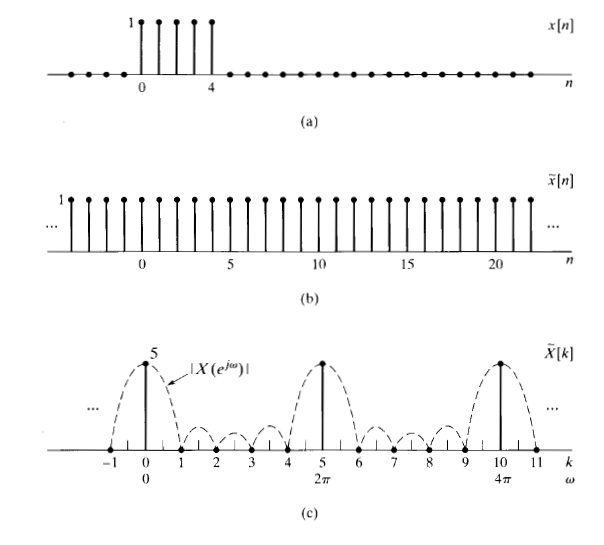
\includegraphics[scale = 0.50]{Figuras/fig810abcOppenheim2aEdicao}
\end{figure}
\end{frame}

%%%

\begin{frame}[c, allowframebreaks]

\textbullet \hspace{0.1cm} \alert{Fazendo $N = 10$}

\begin{figure}[H]
	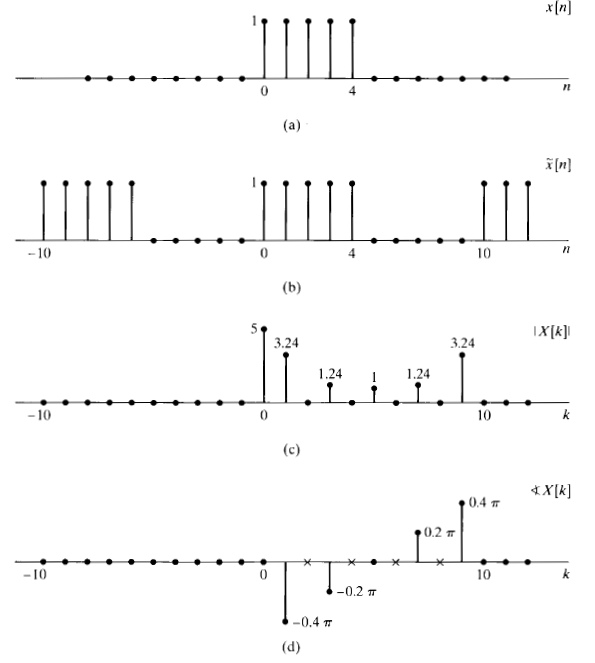
\includegraphics[scale = 0.4]{Figuras/fig811Oppenhiem2aEdicao}
\end{figure}
\end{frame}


%%%
\begin{frame}[c, allowframebreaks]

\textbullet \hspace{0.1cm} \alert{Deslocamento Circular de uma sequência}

\begin{itemize}
\item Se $X(e^{j\omega})$ é a Transforma de Fourier no Tempo Discreto de $x[n]$, então $e^{-j\omega n}X(e^{j\omega n})$ é a Transformada de Fourier de $x[n-m]$.
\item Entretanto, definimos a Transformada Discreta de Fourier $X[k]$ para um sequência finita, logo não faz sentido em falar que $e^{-j\frac{2\pi k}{N}m}X[k]$ não pode ser Transformada de $x[n]$ deslocada, pois o resultado tem que ser de tamanho $N$.
\item Nesse caso, o deslocamento é circular, ou seja, obtém-se o sinal $x_1[n] = x[(n-m)\mod N]$
\end{itemize}

\end{frame}

%%%
\begin{frame}[c, allowframebreaks]

\textbullet \hspace{0.1cm} \alert{Deslocamento Circular de uma sequência}

\begin{figure}[H]
	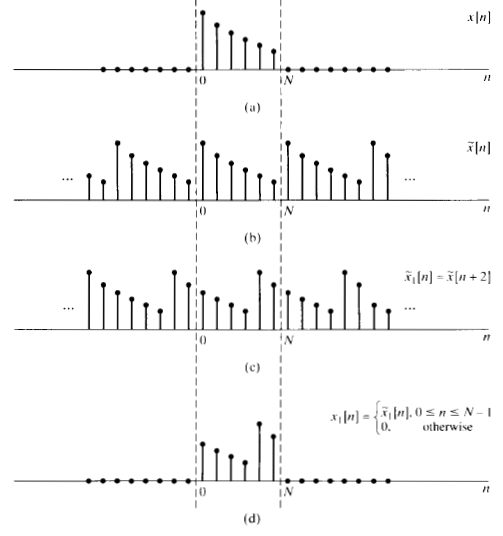
\includegraphics[scale = 0.35]{Figuras/fig812Oppenheim2aEdicao}
\end{figure}

\end{frame}

%%%
\begin{frame}[c, allowframebreaks]

\textbullet \hspace{0.1cm} \alert{Convolução Circular}

\begin{itemize}
\item Da mesma forma que ocorre o deslocamento circular, a convolução de $x_1[n]$ com $x_2[n]$ para obter $x_3[n]$, na frequência dada por $X_3[k] = X_1[k]X_2[k]$ é circular, e dada por
\[
x_3[n]  =\sum\limits_{m=0}^{N-1}x_1[m]x_2[(n-m)\mod N]
\]
\item Exemplo: $x_1[n] = \delta[n - n_0]$, e sinal mostrado abaixo
\begin{figure}[H]
	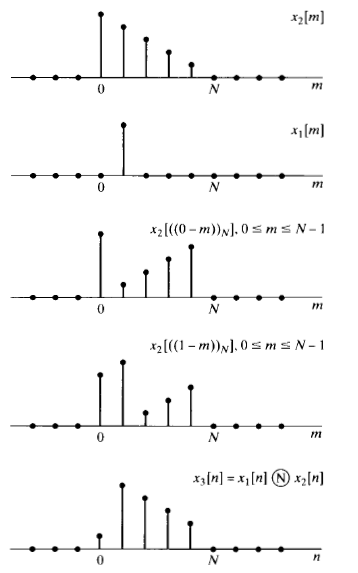
\includegraphics[scale = 0.38]{Figuras/fig814Oppenheim2aEdicao}
\end{figure}
\end{itemize}

\end{frame}

%%%
\begin{frame}[c, allowframebreaks]

\textbullet \hspace{0.1cm} \alert{Convulação Linear Usando a Transformada Discreta de Fourier.}

\begin{itemize}
\item Pode se implementada fazendo:
\begin{enumerate}
\item Calcular a DFT de $N$ pontos $X_1[k]$ e $X_2[k]$ das seuqências $x_1(n)$ e $x_2(n)$.
\item Calcular o produto $X_3[k] = X_1[k]X_2[k]$ para $ 0 \leq k \leq N-1$.
\item Calcule a DFT inversa de $X_3[k]$ para obter $x_3[n]$.
\end{enumerate}
\item A questão é como garantir que a convolução circular tem o mesmo efeito da convolução linear.
\end{itemize}
\end{frame}

%%%
\begin{frame}[c, allowframebreaks]

\textbullet \hspace{0.1cm} \alert{Convolução Linear Usando a Transformada Discreta de Fourier.}

Slides Paulo Diniz

\end{frame}


%%%
\begin{frame}[c, allowframebreaks]

\textbullet \hspace{0.1cm} \alert{FFT e Janelamento}

\begin{itemize}
\item Devemos lembrar que realizamos a DFT de um sinal limitado no tempo, que por sua vez pode ser representado por 
\[
x_N[n]  = x[n]\{u[n] - u[n -N]{
\]
\item Chamaremos a função $w[n] = u[n] - u[n - N]$ de janela.
\item Logo a DFT de $x[n]$ será uma convlução de $xXk]$ com a $W[k]$.
\item Exemplo: sendo $x[n] = cos(\frac{2*\pi n}{16})$ esperamos que seja composto de dois impulsos.
\item Lembrando do efeito da convolução, observamos um espectro ``espalhado'', o que chamamos de DFT {\em leakage} (vazamento).
\end{itemize}
\end{frame}

%%%
\begin{frame}[c, allowframebreaks]

\textbullet \hspace{0.1cm} \alert{FFT e Janelamento}

\begin{itemize}
\item A escolha da janela $w[n]$ é a operação chamada de {\bf janelamento}, e influencia diretamente no resultado da DFT.
\item Alguns tipos de Janelas:
	\begin{itemize}
	\item Retangular: $w[n] = 1,\ n=0,1,2,..., N-1$
	\item Hanning $w[n] = 0.5 - 0.5\cos\left(\frac{2\pi n}{N}\right),\ n=0,1,2,...,N-1$
	\item Hamming $w[n] = 0.54 - 0.46*\cos\left(\frac{2\pi n}{N}\right),\ n=1,2,...,N-1$
	\end{itemize}
\end{itemize}
\end{frame}
\end{document}
%%%
\begin{frame}[c, allowframebreaks]

\textbullet \hspace{0.1cm} \alert{Reduzindo a taxa de amostragem por um fator inteiro.}

\begin{itemize}
\item Na frequência temos que
\[
X(e^{j\omega}) = \frac{1}{T}\sum_{k=-\infty}^{\infty}X_c\left(j\left(\frac{\omega}{T} - \frac{2\pi k}{T}\right)\right)
\]
\item Para $x_d[n] = x[nM] = x_c(NT_1)$, tem-se $T_1 = MT$, logo
\[
x_d(e^{j\omega}) =\frac{1}{T_1}\sum_{r=-\infty}^{\infty}X_c\left(j\left(\frac{\omega}{T_1} - \frac{2\pi k}{T_1}\right)\right)
\]
\end{itemize}
Relacionando essa equações (ver demontração no livro) chega-se a 
\[
X_d(e^{j\omega}) = \frac{1}{M}\sum_{i=0}^{M-1}X(e^{j(\omega/M - 2\pi i/M)})
\]
\end{frame}

%%%
\begin{frame}[c, allowframebreaks]

\textbullet \hspace{0.1cm} \alert{Reduzindo a taxa de amostragem por um fator inteiro.}
Então:
\begin{itemize}
\item $X_d(e^{j\omega})$ é composta de um conjunto infinito de cópias de $X_c(j\Omega)$, escalonadas por $\omega = \Omega T_1$ e descolada por múltiplos inteiro de $2\pi/T_1$
\item Ou ainda, $M$ cópias de $X(e^{j\omega})$ escolonadas na frequência por $M$ e deslocada por múltiplos inteiros de $2\pi$.
\item Como $X_d(e^{j\omega})$ é periodica com período $2\pi$, para que não haja {\em aliasing}
\[
X(e^{j\omega}) = 0,\ \ \omega_N \leq |\omega| \leq \pi
\]
e $2\pi/M \geq 2\omega_N$.
\end{itemize}
\end{frame}

%%%
\begin{frame}[c, allowframebreaks]

\textbullet \hspace{0.1cm} \alert{Reduzindo a taxa de amostragem por um fator inteiro.}

\begin{figure}[H]
	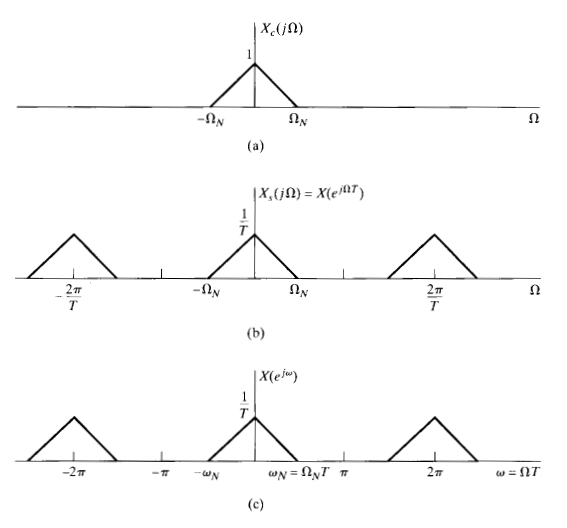
\includegraphics[scale = 0.45]{Figuras/fig421abcOppenheim2aEdicao}
\end{figure}
\end{frame}

%%%
\begin{frame}[c, allowframebreaks]

\textbullet \hspace{0.1cm} \alert{Reduzindo a taxa de amostragem por um fator inteiro.}

\begin{figure}[H]
	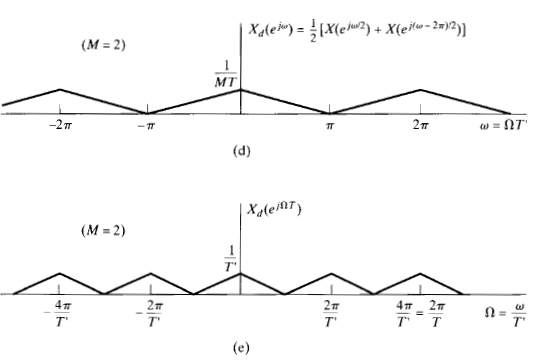
\includegraphics[scale = 0.5]{Figuras/fig421deOppenheim2aEdicao}
\end{figure}
\end{frame}

%%%
\begin{frame}[c, allowframebreaks]

\textbullet \hspace{0.1cm} \alert{Reduzindo a taxa de amostragem por um fator inteiro.}

\begin{figure}[H]
	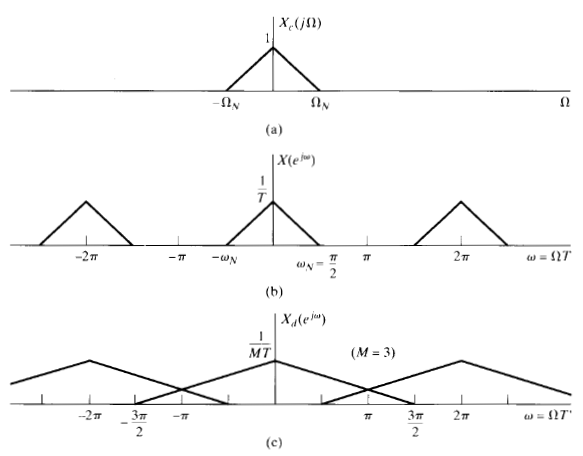
\includegraphics[scale = 0.5]{Figuras/fig422abcOppenheim2aEdicao}
\end{figure}
\end{frame}

%%%
\begin{frame}[c, allowframebreaks]

\textbullet \hspace{0.1cm} \alert{Reduzindo a taxa de amostragem por um fator inteiro.}

\begin{figure}[H]
	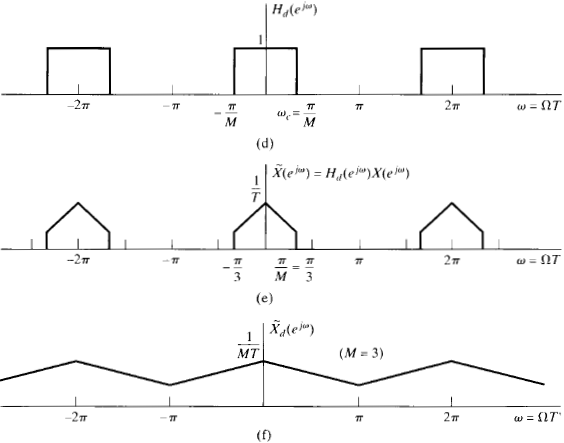
\includegraphics[scale = 0.5]{Figuras/fig422defOppenheim2aEdicao}
\end{figure}
\end{frame}


%%%
\begin{frame}[c, allowframebreaks]

\textbullet \hspace{0.1cm} \alert{Aumentando a taxa de amostragem por um fator inteiro.}

\begin{itemize}
\item Dado um sinal $x[n]$, para aumentar a taxa de amostragem por um fator $L$, obtendo um sinal $x_i[n] = x_c(nT_2)$, sendo $T_2 = T/L$, temos
\[
x_i[n] = x[n/L] x_c(NT/L), n = 0, \pm L, \pm 2L, ...
\]
\item Para obter $x_i[n]$ pode-se usar um sistema
\begin{figure}[H]
	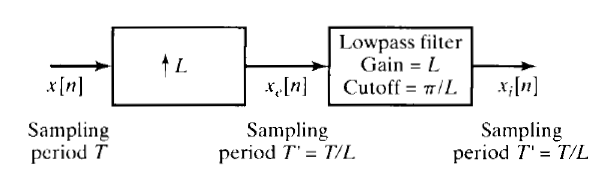
\includegraphics[scale = 0.5]{Figuras/fig424Oppeneheim2aEdicao}
\end{figure}
\end{itemize}

\end{frame}

%%%
\begin{frame}[c, allowframebreaks]

\textbullet \hspace{0.1cm} \alert{Aumentando a taxa de amostragem por um fator inteiro.}

\begin{itemize}
\item Sendo 
\[
x_e[n] = \left\{\begin{array}{c c} x[n/L], & n = 0, \pm L, \pm 2L, ... \\ 0, & c.c. \end{array}\right.
\]
\item ou ainda $x_e[n] = \sum_{k=-\infty}^{\infty}x[k]\delta[n - kL]$.
\item Veja que 
\begin{eqnarray}
X_e(e^{jomega}) &=& \sum_{n=-\infty}^{\infty}\left(\sum_{k=-infty}^{\infty}x[k]\delta[n - kL]\right)e^{-j\omega n} \nonumber \\
&=& \sum_{k=-\infty}^{]infty}x[k]e^{j\omega L k} = X(e^{j\omega L}) \nonumber
\end{eqnarray}
\end{itemize}

\end{frame}

%%%
\begin{frame}[c, allowframebreaks]

\textbullet \hspace{0.1cm} \alert{Aumentando a taxa de amostragem por um fator inteiro.}

\begin{figure}[H]
	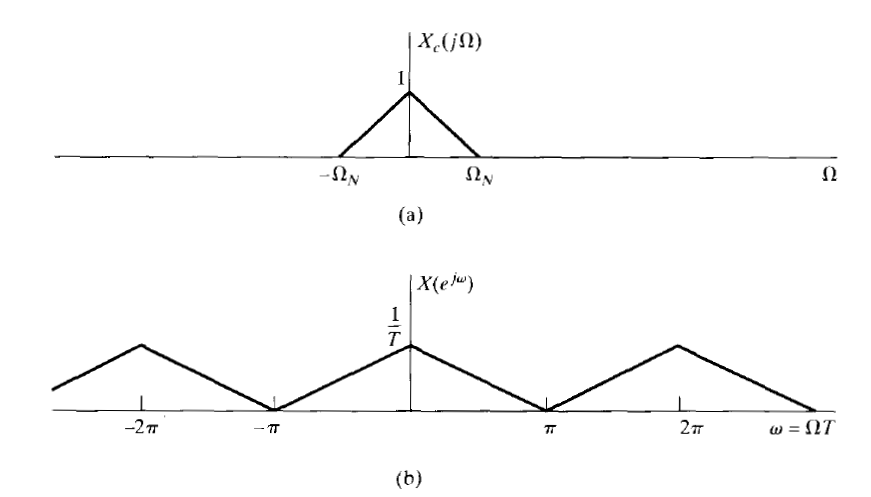
\includegraphics[scale = 0.3]{Figuras/fig425abOppenheim2aEdicao}
\end{figure}

\end{frame}


%%%
\begin{frame}[c, allowframebreaks]

\textbullet \hspace{0.1cm} \alert{Aumentando a taxa de amostragem por um fator inteiro.}

\begin{figure}[H]
	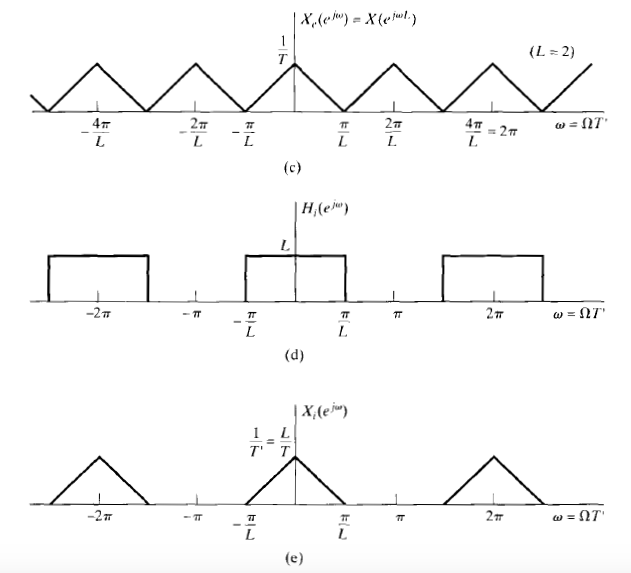
\includegraphics[scale = 0.3]{Figuras/fig425cdeOppenheim2aEdicao}
\end{figure}

\end{frame}

\section{Processamento Digital}

%%%
\begin{frame}[c, allowframebreaks]

\textbullet \hspace{0.1cm} \alert{Filtragem anti-aliasing.}

\begin{itemize}
\item Sinal de entrada não seja limitado em banda, ou taca de Nyquist necessária é muito alta;
\item Filtrar o sinal;
\item Ex.: Sinal de voz, sinal da rede elétrica;
\item Filtro passa baixas:
\[
H(j\Omega) = \left\{\begin{array}{c c} 1, & |\Omega| < \Omega_c  \\ 0, & |\Omega| > \Omega_c \end{array}\right.
\]
\item Pergunta: Já temos um sistema digital? Se não, o que precisamos fazer?
\end{itemize}

\end{frame}


%%%
\begin{frame}[c, allowframebreaks]

\textbullet \hspace{0.1cm} \alert{Conversão Analógico-Digital.}

\begin{itemize}
\item Para obter um sinal digital, podemos utilizar 
\begin{figure}[H]
	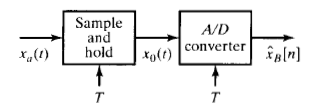
\includegraphics[scale = 0.5]{Figuras/fig445Oppenheim2aEdicao}
\end{figure}
\item Sendo $x_0(t) = \sum_{n=-\infty}^{\infty}x[n]h_0(t - nT)$ com
\[
h_0(t) = \left\{\begin{array}{c c} 1, & 0 < t < T \\ 0, & c.c \end{array} \right.
\]
\end{itemize}

\end{frame}

%%%
\begin{frame}[c, allowframebreaks]

\textbullet \hspace{0.1cm} \alert{Conversão Analógico-Digital.}

\begin{figure}[H]
	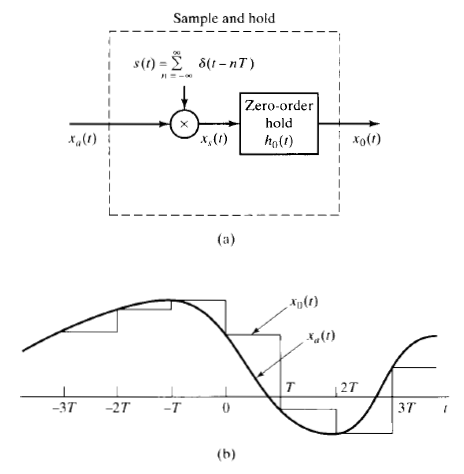
\includegraphics[scale = 0.4]{Figuras/fig446Oppenheim2aEdicao}
\end{figure}

\end{frame}



%%%
\begin{frame}[c, allowframebreaks]

\textbullet \hspace{0.1cm} \alert{Conversão Analógico-Digital - Quantizador.}

\begin{itemize}
\item Sistema não linear para converter as amostras $x[n]$ em valores de um conjunto finito, ou seja, $\hat{x} = Q(x[n])$.
\item Erro de quantização.
\end{itemize}

\begin{figure}[H]
	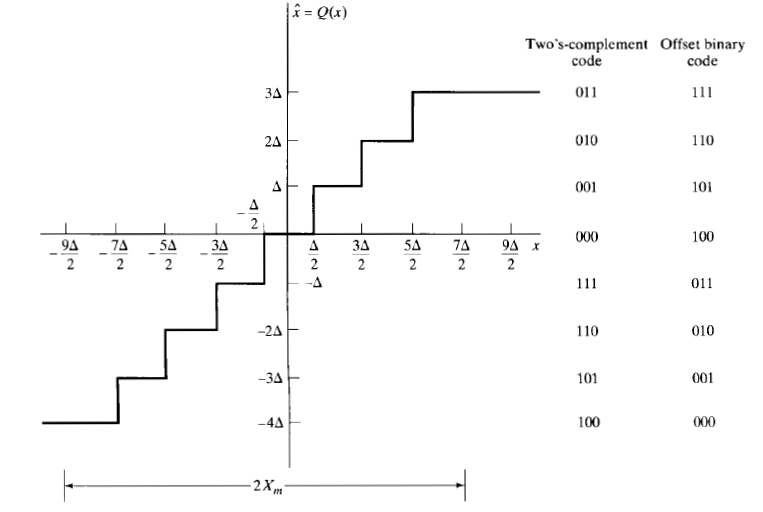
\includegraphics[scale = 0.25]{Figuras/fig448Oppenheim2aEdicao}
\end{figure}

\end{frame}



\section{Amostragem}

\subsection{Amostragem de Sinais Passa-Faixa}

%%%
\begin{frame}[c, allowframebreaks]

\textbullet \hspace{0.1cm} \alert{Sinais passa-faixa.}

\begin{itemize}
\item Frequência central é diferente de zero. P.ex.: sinal modulados.
\item Tem larguga de Banda $B\ Hz$, e frequência central $f_c\ Hz$, logo para amostrá-los $f_s = 2(f_c + B/2)\ Hz$.
\item Exemplo: Sinal centrado em $f_c = 20MHz$ com lagura de banda $B = 5MHz$, então $f_s \geq 45MHz$.


\begin{figure}[H]
	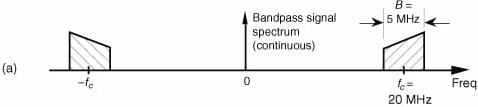
\includegraphics[scale = 0.5]{Figuras/fig27aLyons3aEdicao}
\end{figure}
\item Usando $f_s = 17,5\ MHz$ temos
\end{itemize}
\begin{figure}[H]
	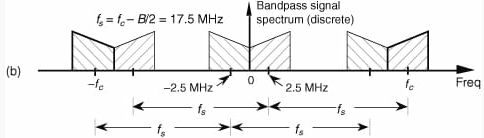
\includegraphics[scale = 0.5]{Figuras/fig27bLyons3aEdicao}
\end{figure}
\end{frame}

\subsection{Amostragem de Sinais Passa-Faixa}

%%%
\begin{frame}[c, allowframebreaks]

\textbullet \hspace{0.1cm} \alert{Amostragem passa-faixas.}

\begin{itemize}
\item Translação por amostragem ({\em sampling translation}).
\item Vantagem?
\item Dá para usar uma taxa ainda menor?
\item Sendo $f_c$ a frequência central, se fizermos
\[
mf_{s2} = 2f_c - B\ ou\ f_{s2} = \frac{2f_c-B}{m}
\]
\begin{figure}[H]
	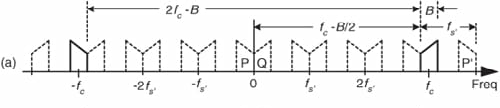
\includegraphics[scale = 0.5]{Figuras/fig28aLyons3aEdicao}
\end{figure}
\end{itemize}
\end{frame}

%%%
\begin{frame}[c, allowframebreaks]

\textbullet \hspace{0.1cm} \alert{Amostragem passa-faixas.}

\begin{figure}[H]
	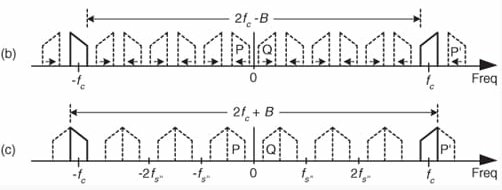
\includegraphics[scale = 0.5]{Figuras/fig28bcLyons3aEdicao}
\end{figure}
\begin{itemize}
\item 
\[
\frac{2f_c-B}{m} \geq  f_{s2} \geq   \frac{2f_c + B}{m+1} 
\]
\end{itemize}
\end{frame}


%%%
\begin{frame}[c, allowframebreaks]

%\textbullet \hspace{0.1cm} \alert{Inversao do Espectro.}
\begin{figure}[H]
	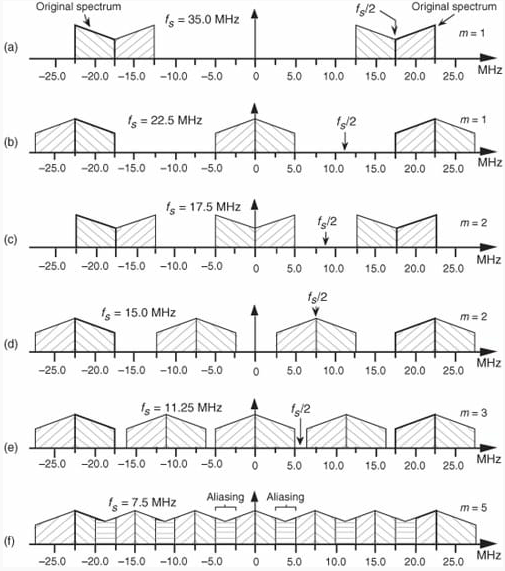
\includegraphics[scale = 0.5]{Figuras/fig29Lyons3aEdicao}
\end{figure}

\end{frame}

%%%
\begin{frame}[c, allowframebreaks]

\textbullet \hspace{0.1cm} \alert{Inversao do Espectro.}
\begin{itemize}
\item Multiplicação por $(-1)^n = \cos(\pi n)$.
\end{itemize}
\begin{figure}[H]
	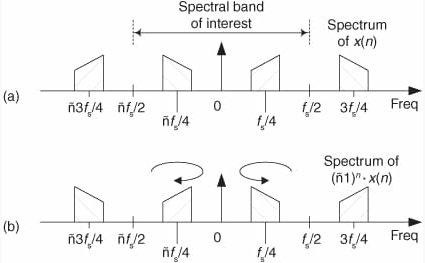
\includegraphics[scale = 0.5]{Figuras/fig210Lyons3aEdicao}
\end{figure}

\end{frame}

%%%
\begin{frame}[c, allowframebreaks]

\textbullet \hspace{0.1cm} \alert{Tarefa:}

\begin{itemize}
\item Utilizando o GNURadio, implemente um sistem para a inversao do esepctro de um sinal de voz tal que:
\begin{enumerate}
\item Leia um sinal wav com uma gravação de voz;
\item Inverta o espectro de frequências dos sinal;
\item Reproduza o sinal com o espectro invertido;
\item Retorno o espectro para a posição original;
\end{enumerate}
\end{itemize}
\end{frame}
\end{document}
